\documentclass[twoside,a4paper]{article}
\usepackage{geometry}
\geometry{margin=1.5cm, vmargin={0pt,1cm}}
\setlength{\topmargin}{-1cm}
\setlength{\paperheight}{29.7cm}
\setlength{\textheight}{25.3cm}

% useful packages.
\usepackage{amsfonts}
\usepackage{amsmath}
\usepackage{amssymb}
\usepackage{amsthm}
\usepackage{enumerate}
\usepackage{graphicx}
\usepackage{multicol}
\usepackage{fancyhdr}
\usepackage{layout}

% some common command
\newcommand{\dif}{\mathrm{d}}
\newcommand{\avg}[1]{\left\langle #1 \right\rangle}
\newcommand{\difFrac}[2]{\frac{\dif #1}{\dif #2}}
\newcommand{\pdfFrac}[2]{\frac{\partial #1}{\partial #2}}
\newcommand{\OFL}{\mathrm{OFL}}
\newcommand{\UFL}{\mathrm{UFL}}
\newcommand{\fl}{\mathrm{fl}}
\newcommand{\op}{\odot}
\newcommand{\Eabs}{E_{\mathrm{abs}}}
\newcommand{\Erel}{E_{\mathrm{rel}}}

\begin{document}

\pagestyle{fancy}
\fancyhead{}
\lhead{NAME Jiatu Yan}
\chead{Numerical Analysis homework \#5}
\rhead{Date}


\section*{I. \small{Run the subroutines on the function $\frac{1}{1+x^2}$.}}

\subsection*{I-a \small{Plot the polynomials.}}

\begin{figure}[h]
	\centering
	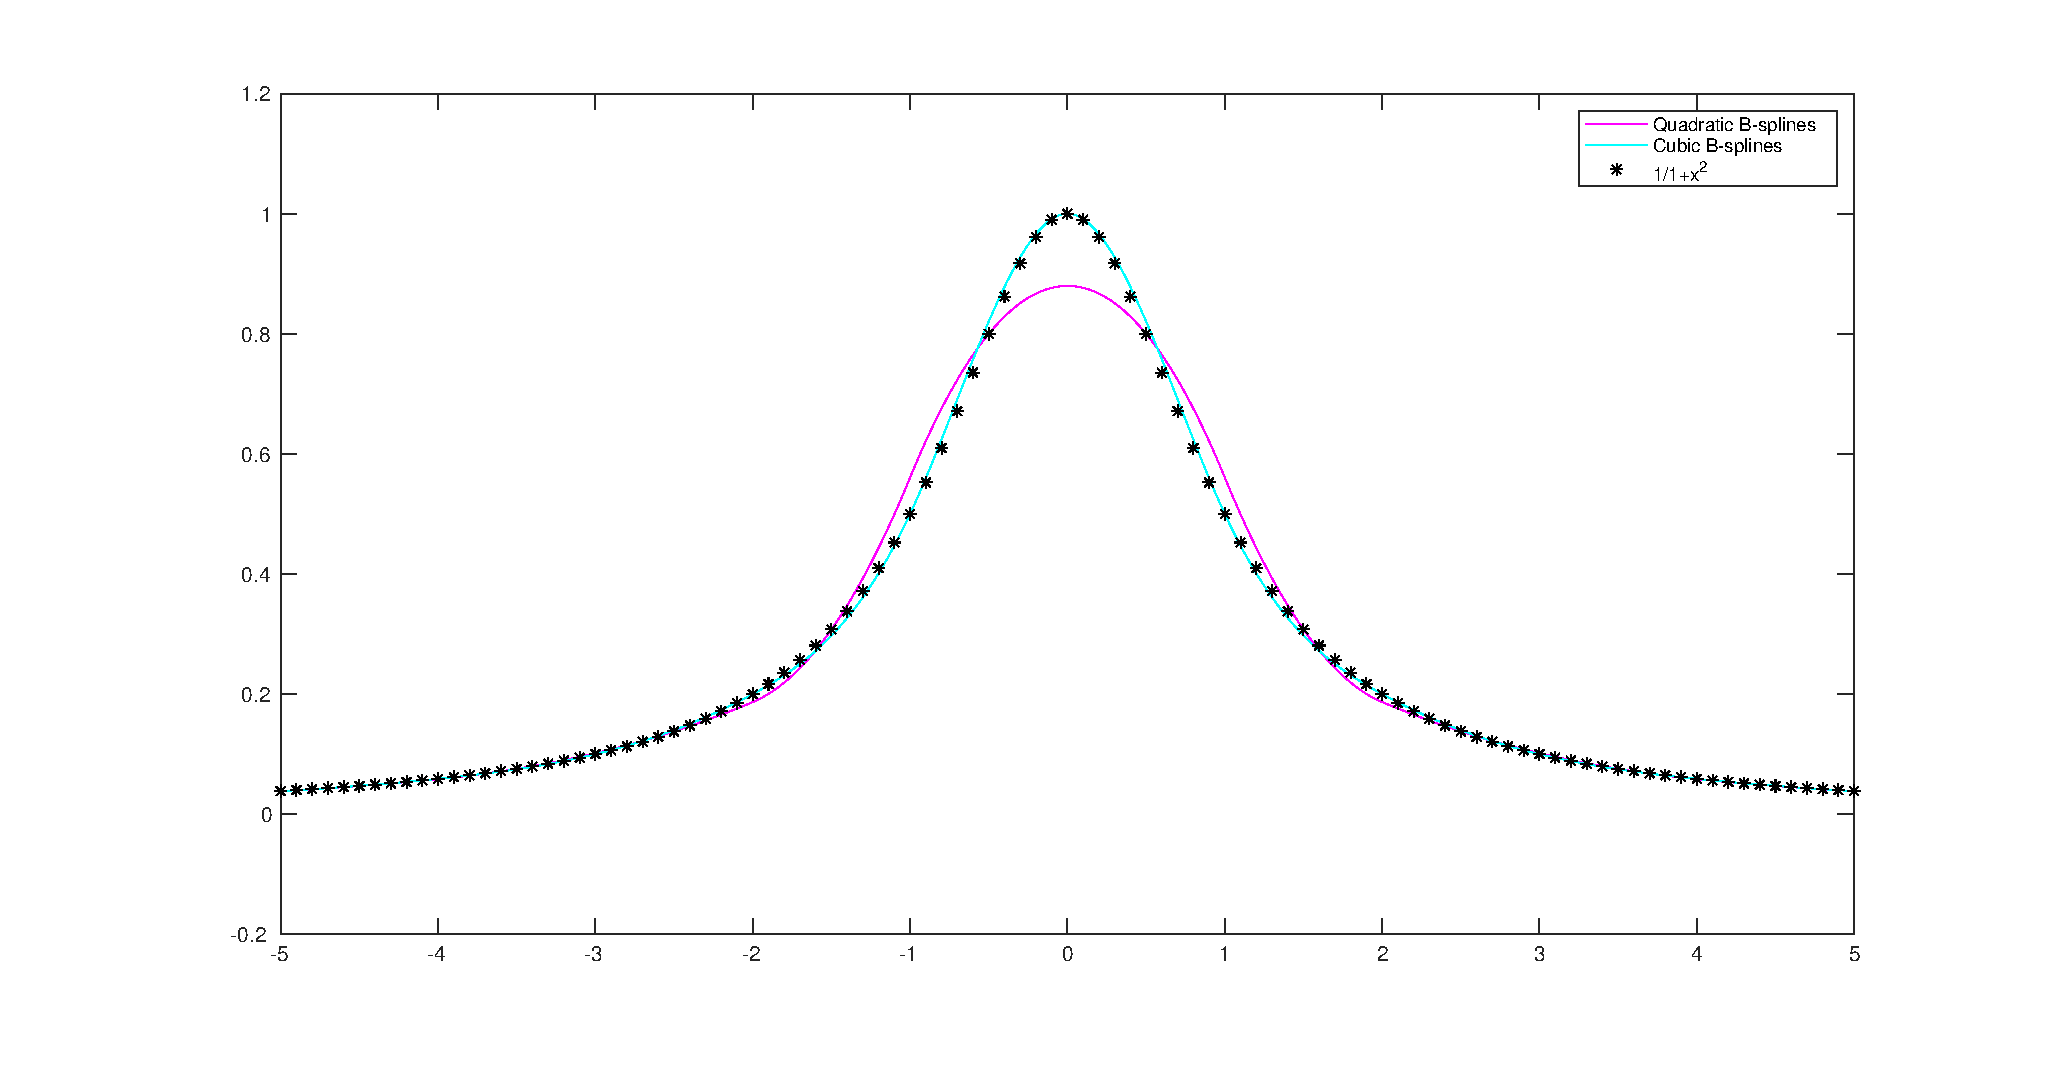
\includegraphics[width=15cm, height=7.5cm]{Bsplines.eps}
	\caption{Interpolating f by quadratic and cubic cardinal B-splines.}
\end{figure}

\subsection*{I-b \small{Consider the $E_{s}(x)$.}}

The $E_s(x)$ of quadratic B-spline interpolants.

\begin{tabular}{|c|c|}
\hline
x&$E_s(x)$\\
\hline
-3.5& 0.000000000000000\\
\hline
-3& 0.001418382673699\\
\hline
-0.5& 0.000000000000000\\
\hline
0& 0.120237781803927\\
\hline
0.5& 0.000000000000000\\
\hline
3& 0.001418382673699\\
\hline
3.5& 0.0000000000000000\\
\hline
\end{tabular}

The $E_s\left( x \right) $ of cubic B-spline interpolants.

\begin{tabular}{|c|c|}
\hline
x&$E_s(x)$\\
\hline
-3.5& 0.000669568235464\\
\hline
-3& 0.000000000000000\\
\hline
-0.5& 0.020528884666179\\
\hline
0& 0.000000000000000\\
\hline
0.5& 0.020528884666179\\
\hline
3& 0.000000000000000\\
\hline
3.5& 0.000669568235464\\
\hline
\end{tabular}

We can find that some errors close to machine precision.
The reason is that the quadratic B-splines interpolant is interpolated by f on $t_i=i-\frac{11}{2}$
, so on -3.5,-0.5,0.5,3.5, the interpolant is absolutely equal to f.
Similarly, quadratic B-splines interpolant is interpolated by f on $t_i=i-6$
, so the error is definitly 0 on -3,0,3.

Although at some points like -3,3, the error of quadratic B-splines interpolants is small
, its maximal error is far larger than that of cubic B-splines. So the cubic B-splines is more accurate.

\section*{II. \small{Plot the heart shape.}}

I choose the complete cubic spline to interpolate the heart shape function.
Since complete cubic spline gurantee the smoothness that $f'\left( a\right)=s'\left( f;a \right)  $ and $f'\left( b \right)=s'\left( f;b \right)  $.

I change the function to $y= \frac{2}{3}(\sqrt{3-t^{4}}+ sign(t)*t),x=t$ and
$y=\frac{2}{3}\left( -\sqrt{3-t^{4}} +sign(t)*t \right)$ and $x= \mid t \mid $,$\left( t\in[0,\sqrt[4]{3} ] \right)$,
I take $\frac{n}{2}$ knots for each of the y function. 
So we can plot the function by taking n knots.

\begin{figure}[ht]
        \centering
        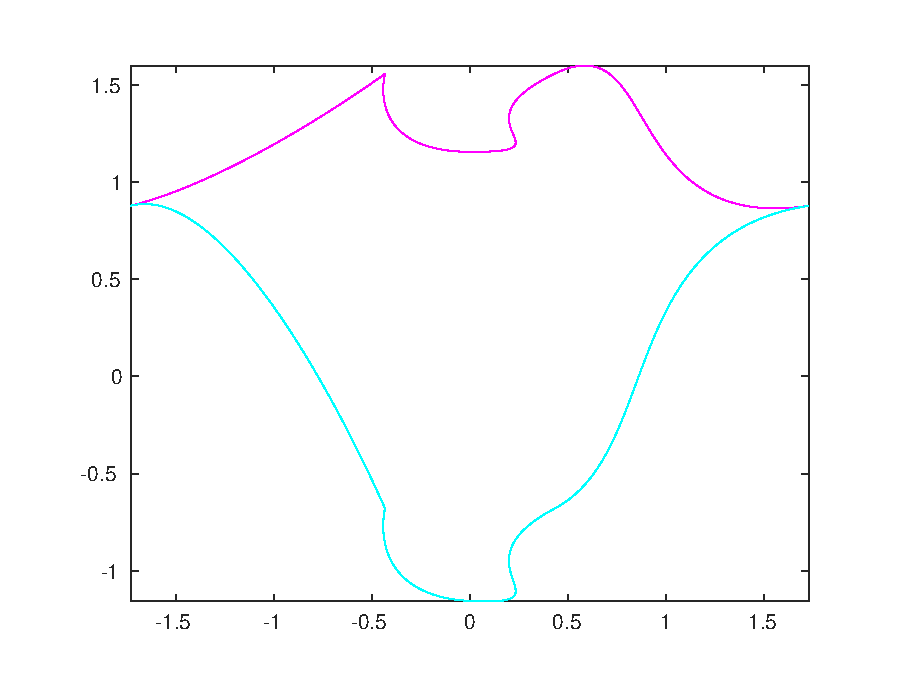
\includegraphics[width=15cm, height=7.5cm]{HeartPlot_10.eps}
        \caption{The interpolants of Heart shape function when n = 10.}
\end{figure}

\begin{figure}[ht]
        \centering
        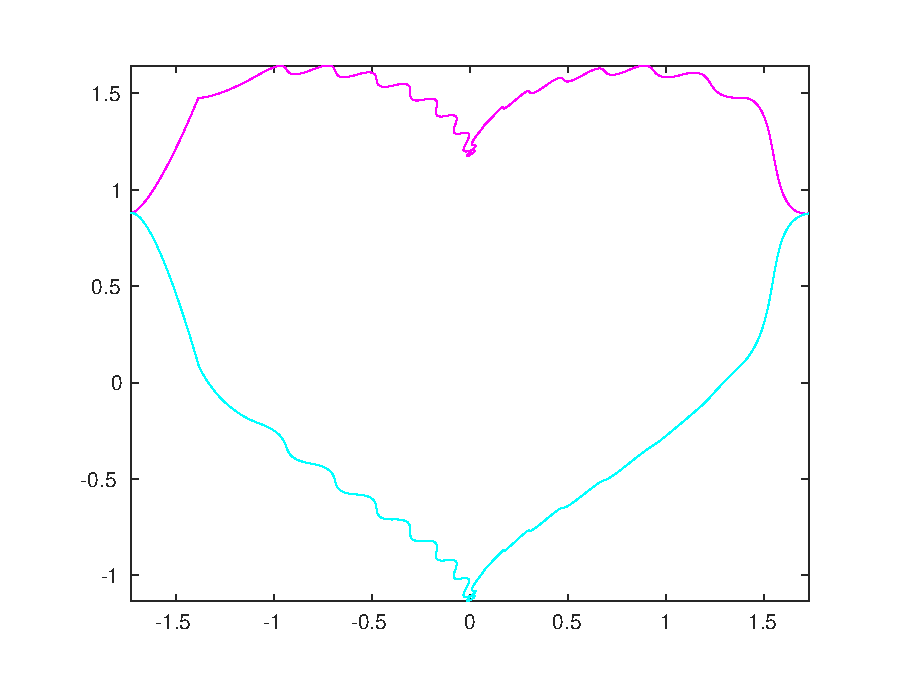
\includegraphics[width=15cm, height=7.5cm]{HeartPlot_40.eps}
        \caption{The interpolants of Heart shape function when n = 40.}
\end{figure}

\begin{figure}[ht]
        \centering
        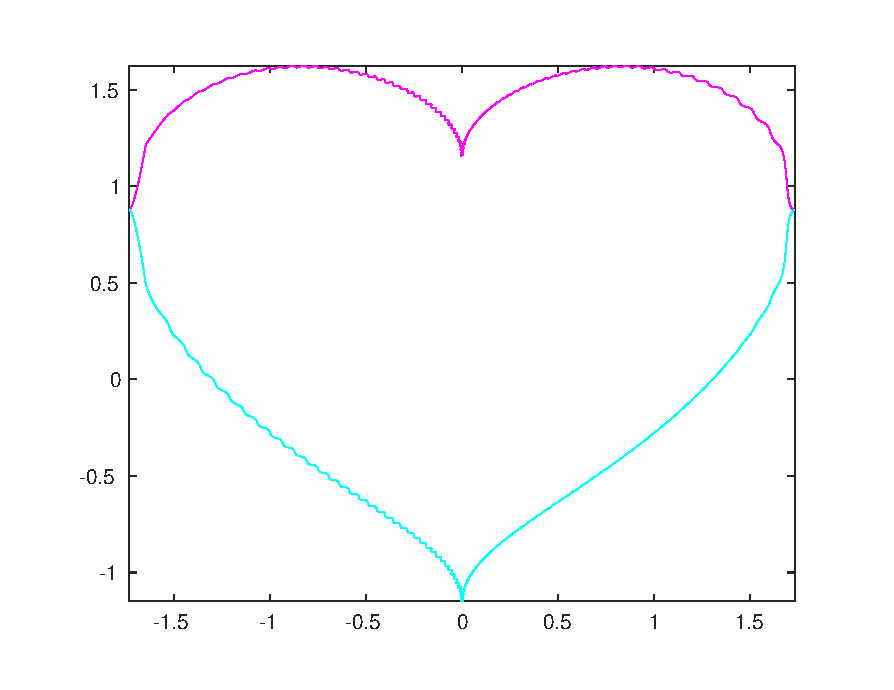
\includegraphics[width=15cm, height=7.5cm]{HeartPlot_160.eps}
        \caption{The interpolants of Heart shape function when n = 160.}
\end{figure}

\end{document}

%%% Local Variables: 
%%% mode: latex
%%% TeX-master: t
%%% End: 
